\begin{frame}[label=title]
    \centering
    \begin{figure}[H]
        
\includegraphics[keepaspectratio, width=0.7\paperwidth, height=\paperheight]{LeeLogo}
    \end{figure}
    Informatik: Data Science und Sicherheit\\
    \emoji{clamp}\textbf{Kompression}
\end{frame}

\begin{frame}[fragile]{Arithmetische Kompression}
\begin{table}[H]
\centering
\begin{tabular}{c|c|c|c|c}
\textbf{Buchstabe} & A & B & C & D \\\hline
\textbf{Häufigkeit (\%)} & 50 & 20 & 20 & 10 \\
\end{tabular}
\end{table}
\newcommand{\arithmeticTikz}[5]{
% 1st argument: height
% 2nd argument: increments
% 3rd argument: xPosL
% 4th argument: xPosR
% 5th argument: letters

	% Draw the initial line
    \draw (0,#1) -- (10,#1);   
	
	% draw 
    \foreach \i in {1,...,4}{
	    \pgfmathsetmacro{\inc}{#2[\i-1]}
	    \pgfmathsetmacro{\l}{#5[\i-1]}
	    \pgfmathsetmacro{\xStart}{#3[\i-1]}
	    \pgfmathsetmacro{\xEnd}{#4[\i-1]}

		% draw vertical marks on main initial line
        \draw (\xStart*10,#1+0.2) to (\xStart*10,#1-0.2);
        \draw (\xEnd*10,#1+0.2) to (\xEnd*10,#1-0.2);
        % annotate interval start & end
        \node (\l-Perc) at (\xStart*10,#1-0.4) {\xStart};
        \node (\l-PercEnd) at (\xEnd*10,#1-0.4) {\xEnd};
        % Increase y position for the next line 
        
        % draw brace and probabilities above line
        \draw[decoration={brace,raise=5pt},decorate]
                (\xStart*10,#1+.2) -- node[above=6pt] {\l{} (\pgfmathparse{int(round(\inc*100))}\pgfmathresult \%)} (\xEnd*10,#1+.2);
    }
}
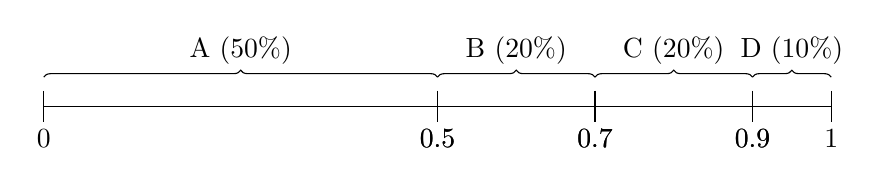
\begin{tikzpicture}
\arithmeticTikz{1}{{0.5,0.2,0.2,0.1}}{{0,0.5,0.7,0.9}}{{0.5,0.7,0.9,1}}{{"A","B","C","D"}}
%\arithmeticTikz{3}{{0.5,0.2,0.2,0.1}}{{0.5,0.6,0.2,0.7}{0,0.5,0.7,0.9}}{{0.5,0.7,0.9,1}}{{"A","B","C","D"}}
 
\end{tikzpicture}
\end{frame}